\section{Theoretical introduction}
This section contains a short theoretical introduction to acoustics. First of all, the wave equation is derived for propagation in a fluid. Secondly, a few essential properties regarding sound reflection, absorption and diffraction are defined. 



\subsection{The wave equation}
The derivation of the wave equation for propagation in a nonviscous fluid is based on Newton's law, the equation of continuity and the adiabatic gas law.


\newpage %hack!!!
\subsubsection{Newton's law}
%\vspace{-15pt}

\begin{wrapfigure}{r}[0.08\textwidth]{0.3\textwidth}
	%\vspace{-60pt}
  \begin{center}
    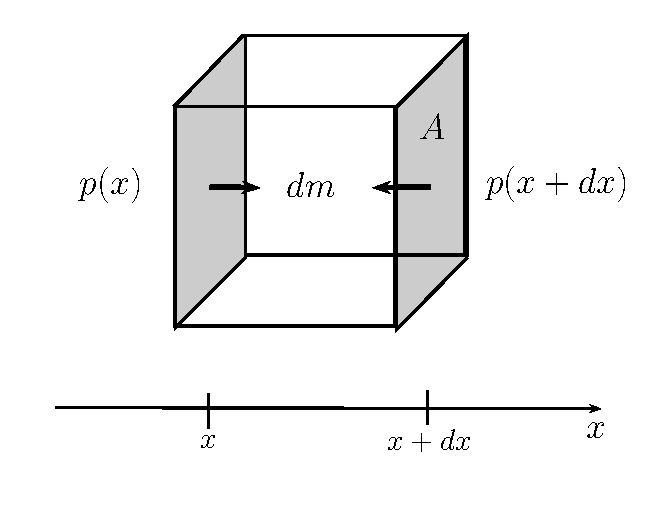
\includegraphics[width=0.3\textwidth]{newton.pdf}
  \end{center}
   %\vspace{-20pt}
  \caption{}\label{fig: newton}
  %\vspace{-20pt}
\end{wrapfigure}

Consider an element of (nonviscous) fluid with mass $dm$ in a volume $A dx$ (see figure \ref{fig: newton}). The force acting in the $x$-direction on surface A at $x$ due to the pressure of the surrounding fluid  is $F(x) = A p(x) $, while the force at $x +dx$ is 
\[
F(x+dx) = - A p(x+dx) = -A [p(x) + \frac{\partial p}{\partial x} dx].
\]
Here the sign is negative since the surrounding fluid pushes the element in the $-x$-direction.
The total $x$-component of the force on mass $dm$ is:
\[
dF_x = F(x) + F(x+dx) = A \left[p(x) - p(x) - \frac{\partial p}{\partial x} dx\right] = - A \frac{\partial p}{\partial x} dx.
\]  
According to Newton's law, this force creates an acceleration of the mass element $dm$:
\[
dF_x = - A \frac{\partial p}{\partial x} dx = \frac{\partial v_x}{\partial t} dm = \rho_0 A \frac{\partial v_x}{\partial t} dx
\]
with $\rho_0$ the static value of the density $\rho$. Simplifying the previous equation and repeating the process for the $y$- and $z$-directions yield
\begin{equation}
\vec{\nabla} p = - \rho_0 \frac{\partial \vec{v}}{\partial t}.
\label{newt}
\end{equation}


\subsubsection{Equation of continuity}
%\vspace{-15pt}
Given that mass is conserved in fluid dynamics, we can write an equation of continuity. Consider a volume element $V$ containing fluid. Any change of mass in $V$ is the result of a flow of particles in or out of this volume element. A change of mass can be written as:
\[
\frac{\partial m}{\partial t} = \frac{\partial }{\partial t} \int_{V} \rho \,dV =\int_{V} \frac{\partial \rho}{\partial t} dV
\]
whereas the flux of particles in or out of the volume is characterised as:
\[
\Phi_m
= - \rho_0 \oint_A \vec{v} \cdot d\vec{A}
= - \rho_0 \int_{V} (\vec{\nabla} \cdot \vec{v}) \, dV.
\]
The divergence theorem was used to obtain the last equality.
Since the change of mass is equal to the mass flux, the following relation between the density and the velocity of the particles can be derived:
\begin{equation}
\frac{\partial \rho}{\partial t}  = - \rho_0 (\vec{\nabla} \cdot \vec{v})
\label{cont}
\end{equation}


\subsubsection{Adiabatic gas law}
%\vspace{-15pt}
It is assumed that the motion of the fluid is an adiabatic process. In combination with the first law of thermodynamics this gives $\delta Q = n C_V dT + p dV = 0$.
If we suppose the fluid to be an ideal gas, following equation holds: $p dV + V dp = n R dT$.
Combining the previous equations gives $\gamma \frac{dV}{V} + \frac{dp}{p} = 0$ with $\gamma \equiv \frac{R+C_V}{C_V} = \frac{C_p}{C_V}$.
Or in terms of the density: $\gamma \frac{d(m/\rho)}{m/ \rho} + \frac{dp}{p} = -\gamma \frac{m}{\rho^2} \frac{d\rho}{m/ \rho} + \frac{dp}{p} =- \gamma \frac{d\rho}{\rho} + \frac{dp}{p} =0$.
In the assumption that the pressure and density variations are small, the equation becomes:
\begin{equation}
\frac{dp}{p_0} =\gamma \frac{d\rho}{\rho_0}
\label{adia}
\end{equation}
with $\rho_0$ the static density and $p_0$ the mean pressure of the surroundings.





\subsubsection{Combination of previous equations}
%\vspace{-15pt}
Combining equations (\ref{cont}) and (\ref{adia}) gives:
\begin{equation}
\frac{\partial p}{\partial t} = - p_0 \gamma \left(\nabla \cdot \vec{v}\right).
\label{dpdt}
\end{equation}
Taking the time derivative of the previous equation and substituting equation (\ref{newt}) gives\\
$\frac{\partial^2 p}{\partial t^2} =  c^2 \Delta p$ with $c\equiv \sqrt{\frac{p_0 \gamma}{\rho_0}}$ the speed of sound in the fluid.







%2.2 Reflection and Absorbtion
%Definition of Reflection coeff and absorbtioncoeff
%Boundary conditions (p_in + p_refl = p_trans and v_n,in + v_n,refl = v_n,trans)
\subsection{Some essential acoustic properties}
In acoustics, several important parameters can be determined in order to characterize the acoustical properties of an object. The  definitions of these parameters are stated in the following paragraphs.


\subsubsection{The reflection coefficient}
%\vspace{-15pt}
When a sound wave travels from one medium to another, it will be reflected and refracted at the boundary surface. Let us consider plane longitudinal waves:
$\pin = \pinnul exp(i (\vec{r} \cdot \kin -  \omega t))$, $\pref = \prefnul exp(i (\vec{r} \cdot \kref -  \omega t))$ and $\ptr = \ptrnul exp(i (\vec{r} \cdot \ktr -  \omega t))$. Let $\thetain$, $\thetaref$ and $\thetatr$ be the angles respective to the normal of the surface of the incoming wave (in), reflected  wave (ref) and transmitted  wave (tr) respectively. The norm of the wave vectors are 
\[
\left\|\kin\right\|
= \left\|\kref\right\|
= \frac{\omega}{c_1}
\qquad\textrm{ and } \qquad
\left\|\ktr\right\|
= \frac{\omega}{c_2}
\]
with $c_1$ and $c_2$ the speeds of sound in medium 1 and 2. The acoustical waves are subject to boundary conditions at the surface. First of all, the law of action and reaction dictates that the pressure should vary continuously at the boundary: $\pin + \pref = \ptr$.
Secondly, the normal velocity of the particles remains the same in both media at the boundary, whereas the tangential component may differ: $\vin^\perp + \vref^\perp = \vtr^\perp$.

These boundary conditions result in Snell's law
\[
\left\|\kin\right\| \sin\thetain = \left\|\kref\right\| \sin\thetaref = \left\|\ktr\right\| \sin\thetatr
\]
and the following solutions in terms of the pressure reflection coefficient $R_p = \prefnul/\pinnul$ and the pressure transmission coefficient $T_p = \ptrnul/\pinnul$ 
\[
R_p = \frac{Z_2 \cos \thetain - Z_1 \cos \thetatr}{Z_2 \cos \thetain + Z_1 \cos \thetatr} \qquad \textrm{ and } \qquad
T_p = \frac{2 Z_2 \cos \thetain }{Z_2 \cos \thetain + Z_1 \cos \thetatr}.
\]
with $Z_1 = \rho_1 c_1$ the characteristic impedance of fluid 1 and $Z_2 = \rho_2 c_2$ the impedance of medium 2.  
The reflection coefficient ranges from $-1$ to 1, while the transmission coefficient has a value between 0 and 2. A value greater than 1 for the transmission coefficient may seem in disagreement with conservation of energy, but that is not the case. We speak of pressure coefficients, instead of intensity coefficients. 

The average acoustic intensity $\vec{I}$ of a sound wave is defined as 
\[
\vec{I} = \frac{1}{T} \int^{T}_{0}{p(t) \vec{v}(t) \,dt}.
\]
with $p$ the instantaneous pressure and $\vec{v}$ the particle velocity. It equals the sound power per unit area. For plane waves, the magnitude of the intensity becomes 
\[
I = \frac{1}{T} \int^{T}_{0}{\frac{\left(p(t)\right)^2}{Z} \,dt} = \frac{p^2_{rms}}{Z}.
\]
The reflection and transmission coefficients are then defined as
\[
R_I = \frac{I_{ref}}{I_{in}} = \frac{p^2_{ref,rms}}{Z_1} \frac{Z_1}{p^2_{in,rms}} = R_p^2 \qquad\textrm{ and } \qquad T_I = \frac{I_{tr}}{I_{in}} = \frac{p^2_{tr,rms}}{Z_2} \frac{Z_1}{p^2_{in,rms}} = T_p^2 \frac{Z_1}{Z_2}. 
\]
When $Z_1 \ll Z_2$, $T_p \approx 2$, but $T_I$ becomes 0. Hence there is no discrepancy.




\subsubsection{The absorption coefficient}
%\vspace{-15pt}
The sound absorption coefficient is defined as the fraction of acoustic energy that is absorbed by the surface on reflection \cite[p.12]{Geetere}.  When dealing with incident plane waves, the absorption coefficient can be written as a function of the (pressure) reflection coefficient:
\begin{equation}
\alpha(\theta_{in}) = 1 - \left|R_p(\theta_{in})\right|^2.
\label{absorption}
\end{equation}




\subsubsection{Diffraction}

A simple rule of thumb is that diffraction effects occur when the dimensions of the obstacle are comparable to the wavelength. A more elaborate rule is given by Rindel\cite{rindel-diffraction} and has been applied by others\cite{davy-diffraction, stage-acoustics}. In the case of an infinite band of height $h$, it states that the diffraction in the far field can be characterized by a frequency $f_0$
\begin{equation}
\label{diffractionEq}
f_0 = \frac{c}{
	\left(\frac{1}{s} + \frac{1}{r}\right) h^2 \cos^2 \theta}
\end{equation}
with $s$ and $r$ the distance from the reflector to the source, respectively to the receiver, and $\theta$ the angle of incidence. For frequencies higher than $f_0$, there is no diffraction. For frequencies lower than $f_0$, the intensity is attenuated by 6dB per octave. 

We will use this formula as a rule of thumb in the measurements of the scale model, even though it only applies in the far field and does not take the floor nor the width of the wall into account. More elaborate solutions that would incorporate these factors and also be valid in the near field are not analytically tractable. Hence the system will be simulated numerically in order to compare measurement with theory.






\begin{comment}
\end{document}
\end{comment}
